\documentclass[]{amsart}
\usepackage[T1]{fontenc}
\usepackage{amssymb,amsmath}
\usepackage{ifxetex,ifluatex}
\usepackage{fixltx2e} % provides \textsubscript
% use upquote if available, for straight quotes in verbatim environments
\IfFileExists{upquote.sty}{\usepackage{upquote}}{}
\ifnum 0\ifxetex 1\fi\ifluatex 1\fi=0 % if pdftex
  \usepackage[utf8]{inputenc}
\else % if luatex or xelatex
  \usepackage{fontspec}
  \ifxetex
    \usepackage{xltxtra,xunicode}
  \fi
  \defaultfontfeatures{Mapping=tex-text,Scale=MatchLowercase}
  \newcommand{\euro}{€}
\fi
% use microtype if available
\IfFileExists{microtype.sty}{\usepackage{microtype}}{}
\usepackage{color}
\usepackage{fancyvrb}
\DefineShortVerb[commandchars=\\\{\}]{\|}
\DefineVerbatimEnvironment{Highlighting}{Verbatim}{commandchars=\\\{\}}
% Add ',fontsize=\small' for more characters per line
\newenvironment{Shaded}{}{}
\newcommand{\KeywordTok}[1]{\textcolor[rgb]{0.00,0.44,0.13}{\textbf{{#1}}}}
\newcommand{\DataTypeTok}[1]{\textcolor[rgb]{0.56,0.13,0.00}{{#1}}}
\newcommand{\DecValTok}[1]{\textcolor[rgb]{0.25,0.63,0.44}{{#1}}}
\newcommand{\BaseNTok}[1]{\textcolor[rgb]{0.25,0.63,0.44}{{#1}}}
\newcommand{\FloatTok}[1]{\textcolor[rgb]{0.25,0.63,0.44}{{#1}}}
\newcommand{\CharTok}[1]{\textcolor[rgb]{0.25,0.44,0.63}{{#1}}}
\newcommand{\StringTok}[1]{\textcolor[rgb]{0.25,0.44,0.63}{{#1}}}
\newcommand{\CommentTok}[1]{\textcolor[rgb]{0.38,0.63,0.69}{\textit{{#1}}}}
\newcommand{\OtherTok}[1]{\textcolor[rgb]{0.00,0.44,0.13}{{#1}}}
\newcommand{\AlertTok}[1]{\textcolor[rgb]{1.00,0.00,0.00}{\textbf{{#1}}}}
\newcommand{\FunctionTok}[1]{\textcolor[rgb]{0.02,0.16,0.49}{{#1}}}
\newcommand{\RegionMarkerTok}[1]{{#1}}
\newcommand{\ErrorTok}[1]{\textcolor[rgb]{1.00,0.00,0.00}{\textbf{{#1}}}}
\newcommand{\NormalTok}[1]{{#1}}
\usepackage{graphicx}
% We will generate all images so they have a width \maxwidth. This means
% that they will get their normal width if they fit onto the page, but
% are scaled down if they would overflow the margins.
\makeatletter
\def\maxwidth{\ifdim\Gin@nat@width>\linewidth\linewidth
\else\Gin@nat@width\fi}
\makeatother
\let\Oldincludegraphics\includegraphics
\renewcommand{\includegraphics}[1]{\Oldincludegraphics[width=\maxwidth]{#1}}
\ifxetex
  \usepackage[setpagesize=false, % page size defined by xetex
              unicode=false, % unicode breaks when used with xetex
              xetex]{hyperref}
\else
  \usepackage[unicode=true]{hyperref}
\fi
\hypersetup{breaklinks=true,
            bookmarks=true,
            pdfauthor={},
            pdftitle={},
            colorlinks=true,
            urlcolor=blue,
            linkcolor=magenta,
            pdfborder={0 0 0}}
\urlstyle{same}  % don't use monospace font for urls
\setlength{\parindent}{0pt}
\setlength{\parskip}{6pt plus 2pt minus 1pt}
\setlength{\emergencystretch}{3em}  % prevent overfull lines
\setcounter{secnumdepth}{5}

\usepackage{times,natbib,bm}

\title[Appendix A: Example \texttt{dsm} analysis]{{\Small Spatial models for distance sampling data:\\ recent developments and future directions}\\ \mbox{} \\Appendix A: Example \texttt{dsm} analysis}

\author{David L. Miller, M. Louise Burt, Eric A. Rexstad and Len Thomas}
\date{}


\begin{document}
\maketitle


\section{Introduction}

The analysis is based on a dataset of observations of pantropical
dolphins in the Gulf of Mexico (shipped with Distance 6.0). For
convenience the data are bundled in an \texttt{R}-friendly format,
although all of the code necessary for creating the data from the
Distance project files is available at the below URL. The OBIS-SEAMAP
page for the data may be found at
\url{http://seamap.env.duke.edu/dataset/25}.

The intention here is to highlight the features of the \texttt{dsm}
package, rather than perform a full analysis of the data. For that
reason, some important steps are not fully explored. Some familiarity
with density surface modelling is assumed.

This is a \texttt{knitr} document. The source for this document contains
everything you need to reproduce the analysis given here (aside from the
data). The most recent version of this document can be found at
\href{http://github.com/dill/mexico-data}{github.com/dill/mexico-data}.

In section 2, we show how the data and packages can be loaded, before moving on to describing the data and then producing some exploratory plots (in sections 3 and 4, respectively). In section 5 we fit a detection function, then a selection of DSMs in section 6. A detection function with covariates is fitted in section 7. An example using correlation structures is shown in section 8, before concluding.

\section{Preamble}

Before we start, we load the \texttt{dsm} package (and its dependencies)
and set some options:

\begin{Shaded}
\begin{Highlighting}[]
\KeywordTok{library}\NormalTok{(dsm)}
\end{Highlighting}
\end{Shaded}

\begin{verbatim}
## Loading required package: mgcv 
## This is mgcv 1.7-24. 
## For overview type 'help("mgcv-package")'.
## Loading required package: mrds 
## Loading required package: optimx
## Loading required package: numDeriv
## Loading required package: Rsolnp
## Loading required package: truncnorm
## Loading required package: parallel
## This is mrds 2.1.1 Built: R 3.0.1; ; 2013-06-25 16:32:18 UTC; unix 
## Loading required package: ggplot2 
## Loading required package: Distance 
## This is dsm 2.0.5 Built: R 3.0.1; ; 2013-06-29 17:14:59 UTC; unix
\end{verbatim}

\begin{Shaded}
\begin{Highlighting}[]

\CommentTok{# plotting options}
\NormalTok{gg.opts <-}\StringTok{ }\KeywordTok{theme}\NormalTok{(}\DataTypeTok{panel.grid.major =} \KeywordTok{element_blank}\NormalTok{(), }
\DataTypeTok{panel.grid.minor =} \KeywordTok{element_blank}\NormalTok{(), }
    \DataTypeTok{panel.background =} \KeywordTok{element_blank}\NormalTok{())}

\CommentTok{# make the results reproducable}
\KeywordTok{set.seed}\NormalTok{(}\DecValTok{11123}\NormalTok{)}
\end{Highlighting}
\end{Shaded}

\section{The data}

\subsection{Observation and segment data}

All of the data for this analysis has been nicely pre-formatted and is
shipped with \texttt{dsm}. Loading up that data, we can see that we have
four data frames, the first few lines of each are shown:

\begin{Shaded}
\begin{Highlighting}[]
\KeywordTok{data}\NormalTok{(mexdolphins)}
\KeywordTok{attach}\NormalTok{(mexdolphins)}
\KeywordTok{head}\NormalTok{(segdata)}
\end{Highlighting}
\end{Shaded}

\begin{verbatim}
##   latitude longitude Effort Transect.Label Sample.Label depth      x
## 1    29.94    -86.93  13800       19960417   19960417-1 135.0 134159
## 2    29.84    -86.83  14000       19960417   19960417-2 147.7 143496
## 3    29.75    -86.74  14000       19960417   19960417-3 152.1 152050
## 4    29.66    -86.65  13900       19960417   19960417-4 163.8 161102
## 5    29.56    -86.57  13800       19960417   19960417-5 179.7 169553
## 6    29.49    -86.49  13800       19960417   19960417-6 188.5 176793
##        y
## 1 325561
## 2 314055
## 3 304324
## 4 293475
## 5 282984
## 6 275103
\end{verbatim}

\begin{Shaded}
\begin{Highlighting}[]
\KeywordTok{head}\NormalTok{(distdata)}
\end{Highlighting}
\end{Shaded}

\begin{verbatim}
##     object size distance Effort detected beaufort latitude longitude
## 45      45   21   3296.6  36300        1        4    27.73    -86.00
## 61      61  150    929.2  17800        1        4    26.00    -87.63
## 63      63  125   6051.0  21000        1        2    26.01    -87.95
## 85      85   75   5499.7  21800        1        1    27.50    -90.45
## 114    114   50   7259.0  13400        1        3    27.41    -94.99
## 120    120   45   1454.8  20900        1        5    26.02    -95.97
##           x       y
## 45   228139   79258
## 61    69199 -113083
## 63    37046 -112197
## 85  -210016   54208
## 114 -658878   43337
## 120 -764824 -111005
\end{verbatim}

\begin{Shaded}
\begin{Highlighting}[]
\KeywordTok{head}\NormalTok{(obsdata)}
\end{Highlighting}
\end{Shaded}

\begin{verbatim}
##     object Sample.Label size distance Effort
## 45      45   19960421-9   21   3296.6  36300
## 61      61   19960423-7  150    929.2  17800
## 63      63   19960423-9  125   6051.0  21000
## 85      85   19960427-1   75   5499.7  21800
## 114    114   19960430-8   50   7259.0  13400
## 120    120   19960501-5   45   1454.8  20900
\end{verbatim}

\begin{Shaded}
\begin{Highlighting}[]
\KeywordTok{head}\NormalTok{(preddata)}
\end{Highlighting}
\end{Shaded}

\begin{verbatim}
##   latitude longitude depth      x      y width height
## 1    30.08    -87.58    35  70832 341079 32072  37065
## 2    30.08    -87.42    30  86868 341079 32072  37065
## 3    30.08    -87.25    27 102904 341079 32072  37065
## 4    30.08    -87.08    22 118940 341079 32072  37065
## 5    30.08    -86.92    46 134976 341079 32072  37065
## 6    29.92    -87.75    14  54888 322546 32126  37065
\end{verbatim}

\texttt{distdata} holds the distance sampling data that will be used to
fit the detection function. \texttt{segdata} holds the segment data: the
transects have already been ``chopped'' into segments. \texttt{obsdata}
holds the observations which have already been aggregated to the
segments and \texttt{preddata} holds the prediction grid (which includes
all the necessary covariates).

Typically (i.e.~for other datasets) it will be necessary divide the
transects into segments, and allocate observations to the correct
segments using a GIS or other similar package, before starting an
analysis using \texttt{dsm}.

\subsection{Converting units}

It is important to ensure that the measurements to be used in the
analysis are in compatible units, otherwise the resulting estimates will
be incorrect or hard to interpret. Having all of our measurements in SI
units from the outset removes the need for conversion later, making life
much easier. All of the data are already in the appropriate units
(Northings and Eastings: kilometres from \textasciitilde{} -88.32
longitude, \textasciitilde{}27.02 latitude, which is the centroid of the
study region, multiplied up by 1000 to get the result in metres, for
consistency).

We give an example of converting the survey area here to show that this
is a simple process:

\begin{Shaded}
\begin{Highlighting}[]
\CommentTok{# centroid}
\NormalTok{lon0 <-}\StringTok{ }\NormalTok{-}\FloatTok{88.31951}
\NormalTok{lat0 <-}\StringTok{ }\FloatTok{27.01594}

\NormalTok{sa.tmp <-}\StringTok{ }\KeywordTok{latlong2km}\NormalTok{(survey.area$longitude, survey.area$latitude, }\DataTypeTok{lon0 =} \NormalTok{lon0, }
    \DataTypeTok{lat0 =} \NormalTok{lat0)}

\NormalTok{survey.area <-}\StringTok{ }\KeywordTok{data.frame}\NormalTok{(}\DataTypeTok{x =} \DecValTok{1000} \NormalTok{*}\StringTok{ }\NormalTok{sa.tmp$km.e, }\DataTypeTok{y =} \DecValTok{1000} \NormalTok{*}\StringTok{ }\NormalTok{sa.tmp$km.n)}

\KeywordTok{rm}\NormalTok{(sa.tmp)}
\end{Highlighting}
\end{Shaded}

The function \texttt{latlong2km} uses the spherical law of cosines to
convert latitude and longitude into Northings and Eastings (thanks to
Simon N. Wood for providing code). There is extensive literature about
when particular projections of latitude and longitude are appropriate
and we highly recommend the reader review this for their particular
study area. The other data frames have already had their measurements
appropriately converted. By convention the directions are named
\texttt{x} and \texttt{y}.

Using latitude and longitude when performing spatial smoothing can be
problematic when certain smoother bases are used. In particular when
bivariate isotropic bases are used the non-isotropic nature of latitude
and longitude is inconsistent (moving one degree in one direction is not
the same as moving one degree in the other).

The below code generates Figure 1, which shows the survey area with the
transect lines overlaid (using data from \texttt{segdata}).

\begin{Shaded}
\begin{Highlighting}[]
\NormalTok{p <-}\StringTok{ }\KeywordTok{qplot}\NormalTok{(}\DataTypeTok{data =} \NormalTok{survey.area, }\DataTypeTok{x =} \NormalTok{x, }\DataTypeTok{y =} \NormalTok{y, }\DataTypeTok{geom =} \StringTok{"polygon"}\NormalTok{, }
	\DataTypeTok{fill =} \KeywordTok{I}\NormalTok{(}\StringTok{"lightblue"}\NormalTok{), }\DataTypeTok{ylab =} \StringTok{"y"}\NormalTok{, }\DataTypeTok{xlab =} \StringTok{"x"}\NormalTok{, }\DataTypeTok{alpha =} \KeywordTok{I}\NormalTok{(}\FloatTok{0.7}\NormalTok{))}
\NormalTok{p <-}\StringTok{ }\NormalTok{p +}\StringTok{ }\KeywordTok{coord_equal}\NormalTok{()}
\NormalTok{p <-}\StringTok{ }\NormalTok{p +}\StringTok{ }\NormalTok{gg.opts}

\NormalTok{p <-}\StringTok{ }\NormalTok{p +}\StringTok{ }\KeywordTok{geom_line}\NormalTok{(}\KeywordTok{aes}\NormalTok{(x, y, }\DataTypeTok{group =} \NormalTok{Transect.Label), }\DataTypeTok{data =} \NormalTok{segdata)}

\KeywordTok{print}\NormalTok{(p)}
\end{Highlighting}
\end{Shaded}

\begin{figure}[htbp]
\centering
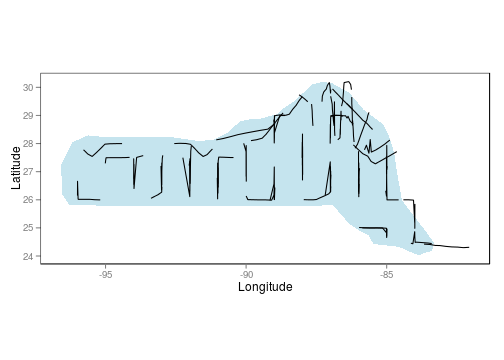
\includegraphics{mexico-figs/areawithtransects.png}
\caption{The survey area with transect lines.}
\end{figure}

\section{Exploratory data analysis}

\subsection{Distance data}

The top panels of Figure 2, below, show histograms of observed distances
and cluster size, while the bottom panels show the relationship between
observed distance and observed cluster size, and the relationship
between observed distance and Beaufort sea state. The plots show that
there is some relationship between cluster size and observed distance
(fewer smaller clusters seem to be seen at larger distances).

The following code generates Figure 2:

\begin{Shaded}
\begin{Highlighting}[]
\KeywordTok{par}\NormalTok{(}\DataTypeTok{mfrow =} \KeywordTok{c}\NormalTok{(}\DecValTok{2}\NormalTok{, }\DecValTok{2}\NormalTok{))}

\CommentTok{# histograms}
\KeywordTok{hist}\NormalTok{(distdata$distance, }\DataTypeTok{main =} \StringTok{""}\NormalTok{, }\DataTypeTok{xlab =} \StringTok{"Distance (m)"}\NormalTok{)}
\KeywordTok{hist}\NormalTok{(distdata$size, }\DataTypeTok{main =} \StringTok{""}\NormalTok{, }\DataTypeTok{xlab =} \StringTok{"Cluster size"}\NormalTok{)}

\CommentTok{# plots of distance vs. cluster size}
\KeywordTok{plot}\NormalTok{(distdata$distance, distdata$size, }\DataTypeTok{main =} \StringTok{""}\NormalTok{, }\DataTypeTok{xlab =} \StringTok{"Distance (m)"}\NormalTok{, }
    \DataTypeTok{ylab =} \StringTok{"Group size"}\NormalTok{, } \DataTypeTok{pch =} \DecValTok{19}\NormalTok{, }\DataTypeTok{cex =} \FloatTok{0.5}\NormalTok{, }\DataTypeTok{col =} \KeywordTok{rgb}\NormalTok{(}\FloatTok{0.74}\NormalTok{, }\FloatTok{0.74}\NormalTok{, }\FloatTok{0.74}\NormalTok{, }\FloatTok{0.7}\NormalTok{))}

\CommentTok{# lm fit}
\NormalTok{l.dat <-}\StringTok{ }\KeywordTok{data.frame}\NormalTok{(}\DataTypeTok{distance =} \KeywordTok{seq}\NormalTok{(}\DecValTok{0}\NormalTok{, }\DecValTok{8000}\NormalTok{, }\DataTypeTok{len =} \DecValTok{1000}\NormalTok{))}
\NormalTok{lo <-}\StringTok{ }\KeywordTok{lm}\NormalTok{(size ~}\StringTok{ }\NormalTok{distance, }\DataTypeTok{data =} \NormalTok{distdata)}
\KeywordTok{lines}\NormalTok{(l.dat$distance, }\KeywordTok{as.vector}\NormalTok{(}\KeywordTok{predict}\NormalTok{(lo, l.dat)))}

\KeywordTok{plot}\NormalTok{(distdata$distance, distdata$beaufort, }\DataTypeTok{main =} \StringTok{""}\NormalTok{, }\DataTypeTok{xlab =} \StringTok{"Distance (m)"}\NormalTok{, }
    \DataTypeTok{ylab =} \StringTok{"Beaufort sea state"}\NormalTok{, }\DataTypeTok{pch =} \DecValTok{19}\NormalTok{, }\DataTypeTok{cex =} \FloatTok{0.5}\NormalTok{, }\DataTypeTok{col =} \KeywordTok{rgb}\NormalTok{(}\FloatTok{0.74}\NormalTok{, }\FloatTok{0.74}\NormalTok{, }
        \FloatTok{0.74}\NormalTok{, }\FloatTok{0.7}\NormalTok{))}
\end{Highlighting}
\end{Shaded}

\begin{figure}[htbp]
\centering
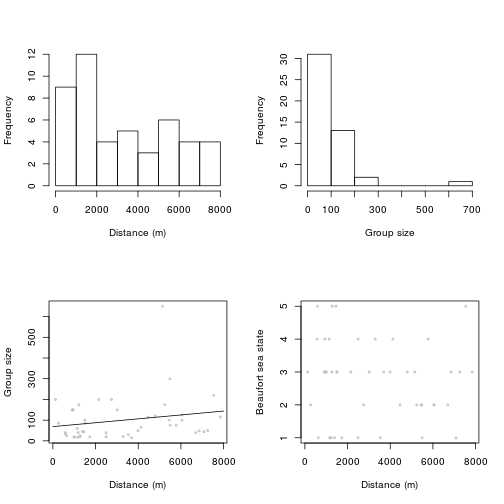
\includegraphics{mexico-figs/EDA-plots.png}
\caption{Exploratory plot of the distance sampling data. Top row, left
to right: histograms of distance and cluster size; bottom row: plot of
distance against cluster size and plot of distances against Beaufort sea
state.}
\end{figure}

\subsection{Spatial data}

Looking separately at the spatial data without thinking about the
distances, we can see the distribution of group size in space in Figure
3, below. Circle size indicates the size of the group in the
observation. There are rather large areas with no observations, which
might cause our variance estimates to be rather large. This plot shows
that we don't seem to have many observations in the very shallow areas
near the shore. This should make us skeptical of predictions in those
areas. We will use depth later as an explanatory covariate in our
spatial model. Figure 3 also shows the raw depth data.

The following code generates Figure 3:

\begin{Shaded}
\begin{Highlighting}[]
\NormalTok{p <-}\StringTok{ }\KeywordTok{ggplot}\NormalTok{(preddata)}
\NormalTok{p <-}\StringTok{ }\NormalTok{p +}\StringTok{ }\NormalTok{gg.opts}
\NormalTok{p <-}\StringTok{ }\NormalTok{p +}\StringTok{ }\KeywordTok{coord_equal}\NormalTok{()}
\NormalTok{p <-}\StringTok{ }\NormalTok{p +}\StringTok{ }\KeywordTok{labs}\NormalTok{(}\DataTypeTok{fill =} \StringTok{"Depth"}\NormalTok{, }\DataTypeTok{x =} \StringTok{"x"}\NormalTok{, }\DataTypeTok{y =} \StringTok{"y"}\NormalTok{, }\DataTypeTok{size =} \StringTok{"Group size"}\NormalTok{)}
\NormalTok{p <-}\StringTok{ }\NormalTok{p +}\StringTok{ }\KeywordTok{geom_tile}\NormalTok{(}\KeywordTok{aes}\NormalTok{(}\DataTypeTok{x =} \NormalTok{x, }\DataTypeTok{y =} \NormalTok{y, }\DataTypeTok{fill =} \NormalTok{depth, }
    \DataTypeTok{width =} \NormalTok{width, }\DataTypeTok{height =} \NormalTok{height))}
\NormalTok{p <-}\StringTok{ }\NormalTok{p +}\StringTok{ }\KeywordTok{geom_line}\NormalTok{(}\KeywordTok{aes}\NormalTok{(x, y, }\DataTypeTok{group =} \NormalTok{Transect.Label), }\DataTypeTok{data =} \NormalTok{segdata)}
\NormalTok{p <-}\StringTok{ }\NormalTok{p +}\StringTok{ }\KeywordTok{geom_point}\NormalTok{(}\KeywordTok{aes}\NormalTok{(x, y, }\DataTypeTok{size =} \NormalTok{size), }\DataTypeTok{data =} \NormalTok{distdata, }\DataTypeTok{colour =} \StringTok{"red"}\NormalTok{, }
    \DataTypeTok{alpha =} \KeywordTok{I}\NormalTok{(}\FloatTok{0.7}\NormalTok{))}
\KeywordTok{print}\NormalTok{(p)}
\end{Highlighting}
\end{Shaded}

\begin{figure}[htbp]
\centering
\includegraphics{mexico-figs/unnamed-chunk-4.png}
\caption{Plot of depth values over the survey area with transects and
observations overlaid. Point size is proportional to the group size for
each observation.}
\end{figure}

\section{Estimating the detection function}

We use the \texttt{ds} function in the package \texttt{Distance} to fit
the detection function. (The \texttt{Distance} package is intended to
make standard distance sampling in \texttt{R} relatively
straightforward. For a more flexible, but harder to use, alternaitve,
see the function \texttt{ddf} in the \texttt{mrds} library.)

First, loading the \texttt{Distance} library:

\begin{Shaded}
\begin{Highlighting}[]
\KeywordTok{library}\NormalTok{(Distance)}
\end{Highlighting}
\end{Shaded}

We can then fit a detection function with hazard-rate key with no
adjustment terms:

\begin{Shaded}
\begin{Highlighting}[]
\NormalTok{hr.model <-}\StringTok{ }\KeywordTok{ds}\NormalTok{(distdata, }\KeywordTok{max}\NormalTok{(distdata$distance), }\DataTypeTok{key =} \StringTok{"hr"}\NormalTok{, }\DataTypeTok{adjustment =} \OtherTok{NULL}\NormalTok{)}
\end{Highlighting}
\end{Shaded}

\begin{verbatim}
## Fitting hazard-rate key function AIC= 841.253
## No survey area information supplied, only estimating detection function.
\end{verbatim}

\begin{Shaded}
\begin{Highlighting}[]
\KeywordTok{summary}\NormalTok{(hr.model)}
\end{Highlighting}
\end{Shaded}

\begin{verbatim}
## 
## Summary for distance analysis 
## Number of observations :  47 
## Distance range         :  0  -  7847 
## 
## Model : Hazard-rate key function 
## AIC   : 841.3 
## 
## Detection function parameters
## Scale Coefficients:  
##             estimate     se
## (Intercept)    7.983 0.9532
## 
## Shape parameters:  
##             estimate     se
## (Intercept)        0 0.7835
## 
##                     Estimate      SE     CV
## Average p             0.5913  0.2224 0.3762
## N in covered region  79.4879 30.8073 0.3876
\end{verbatim}

The following code generates a plot of the fitted detection function
(Figure 4):

\begin{Shaded}
\begin{Highlighting}[]
\KeywordTok{plot}\NormalTok{(hr.model)}
\end{Highlighting}
\end{Shaded}

\begin{figure}[htbp]
\centering
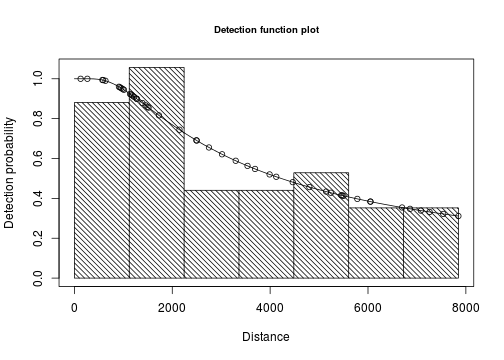
\includegraphics{mexico-figs/hr-detfct.png}
\caption{Plot of the fitted detection function.}
\end{figure}

For brevity, detection function model selection has been omitted here.
In practise we would fit many different forms for the detection
function. Later in this document, we demonstrate fitting of a detection
function with size as a covariate, but for now we stick to a simple
model.

\section{Fitting a DSM}

Before fitting a \texttt{dsm} model, the data must be segmented; this
consists of chopping up the transects and attributing counts to each of
the segments. As mentioned above, these data have already been
segmented.

\subsection{A simple model}

We begin with a very simple model. We assume that the number of
individuals in each segment are quasi-Poisson distributed and that they
are a smooth function of their spatial coordinates (note that the
formula is exactly as one would specify to \texttt{gam} in
\texttt{mgcv}). The abundance of clusters/groups rather than individuals
can be estimated by setting \texttt{group=TRUE} (though we ignore this
here).

Running the model:

\begin{Shaded}
\begin{Highlighting}[]
\NormalTok{mod1 <-}\StringTok{ }\KeywordTok{dsm}\NormalTok{(N ~}\StringTok{ }\KeywordTok{s}\NormalTok{(x, y), hr.model$ddf, segdata, obsdata)}
\KeywordTok{summary}\NormalTok{(mod1)}
\end{Highlighting}
\end{Shaded}

\begin{verbatim}
## 
## Family: quasipoisson 
## Link function: log 
## 
## Formula:
## N ~ s(x, y) + offset(off.set)
## <environment: 0x10a71c2e8>
## 
## Parametric coefficients:
##             Estimate Std. Error t value Pr(>|t|)    
## (Intercept)  -18.409      0.394   -46.7   <2e-16 ***
## ---
## Signif. codes:  0 '***' 0.001 '**' 0.01 '*' 0.05 '.' 0.1 ' ' 1
## 
## Approximate significance of smooth terms:
##         edf Ref.df    F p-value    
## s(x,y) 26.1   28.2 5.61  <2e-16 ***
## ---
## Signif. codes:  0 '***' 0.001 '**' 0.01 '*' 0.05 '.' 0.1 ' ' 1
## 
## R-sq.(adj) =  0.113   Deviance explained =   44%
## GCV score = 42.985  Scale est. = 37.611    n = 387
\end{verbatim}

We can then make the predictions over the the grid and calculate
abundance. First we must create the offset (the area of each grid cell,
which is 444km$^2$).

\begin{Shaded}
\begin{Highlighting}[]
\NormalTok{off.set <-}\StringTok{ }\DecValTok{444} \NormalTok{*}\StringTok{ }\DecValTok{1000} \NormalTok{*}\StringTok{ }\DecValTok{1000}
\NormalTok{mod1.pred <-}\StringTok{ }\KeywordTok{predict}\NormalTok{(mod1, preddata, off.set)}
\end{Highlighting}
\end{Shaded}

Figure 5 shows a map of the predicted abundance. Before plotting, we
bind on the predicitons to the data used to create them:

\begin{Shaded}
\begin{Highlighting}[]
\NormalTok{pp <-}\StringTok{ }\KeywordTok{cbind}\NormalTok{(preddata, mod1.pred)}
\NormalTok{p <-}\StringTok{ }\KeywordTok{ggplot}\NormalTok{(pp) +}\StringTok{ }\NormalTok{gg.opts}
\NormalTok{p <-}\StringTok{ }\NormalTok{p +}\StringTok{ }\KeywordTok{geom_tile}\NormalTok{(}\KeywordTok{aes}\NormalTok{(}\DataTypeTok{x =} \NormalTok{x, }\DataTypeTok{y =} \NormalTok{y, }\DataTypeTok{fill =} \NormalTok{mod1.pred, }
    \DataTypeTok{width =} \NormalTok{width, }\DataTypeTok{height =} \NormalTok{height))}
\NormalTok{p <-}\StringTok{ }\NormalTok{p +}\StringTok{ }\KeywordTok{coord_equal}\NormalTok{()}
\NormalTok{p <-}\StringTok{ }\NormalTok{p +}\StringTok{ }\KeywordTok{geom_path}\NormalTok{(}\KeywordTok{aes}\NormalTok{(}\DataTypeTok{x =} \NormalTok{x, }\DataTypeTok{y =} \NormalTok{y), }\DataTypeTok{data =} \NormalTok{survey.area)}
\NormalTok{p <-}\StringTok{ }\NormalTok{p +}\StringTok{ }\KeywordTok{labs}\NormalTok{(}\DataTypeTok{fill =} \StringTok{"Abundance"}\NormalTok{)}
\KeywordTok{print}\NormalTok{(p)}
\end{Highlighting}
\end{Shaded}

\begin{figure}[htbp]
\centering
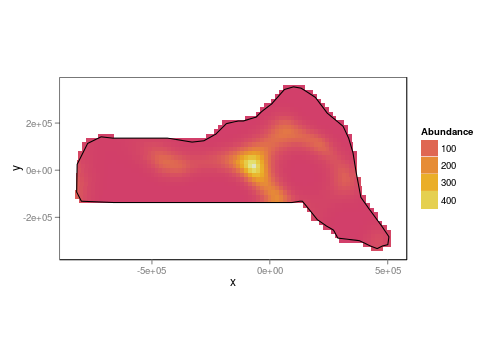
\includegraphics{mexico-figs/mod1-preds.png}
\caption{Predicted density surface for \texttt{mod1}.}
\end{figure}

We can calculate abundance over the survey area by simply summing these
predictions:

\begin{Shaded}
\begin{Highlighting}[]
\KeywordTok{sum}\NormalTok{(mod1.pred)}
\end{Highlighting}
\end{Shaded}

\begin{verbatim}
## [1] 47034
\end{verbatim}

Figure 6 shows diagnostic plots for the model, generated with the
following code:.

\begin{Shaded}
\begin{Highlighting}[]
\KeywordTok{gam.check}\NormalTok{(mod1)}
\end{Highlighting}
\end{Shaded}

\begin{figure}[htbp]
\centering
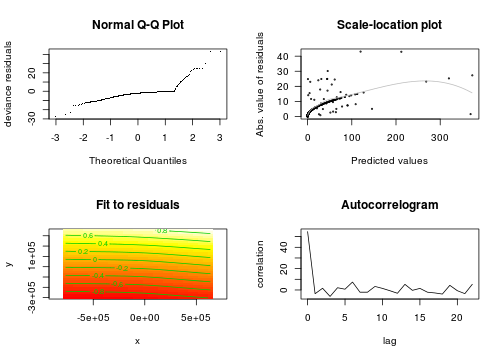
\includegraphics{mexico-figs/mod1-check.png}
\caption{Diagnostic plots for \texttt{mod1}.}
\end{figure}

\begin{verbatim}
## 
## Method: GCV   Optimizer: outer newton
## full convergence after 4 iterations.
## Gradient range [4.281e-07,4.281e-07]
## (score 42.99 & scale 37.61).
## Hessian positive definite, eigenvalue range [0.4516,0.4516].
## 
## Basis dimension (k) checking results. Low p-value (k-index<1) may
## indicate that k is too low, especially if edf is close to k'.
## 
##           k'   edf k-index p-value
## s(x,y) 29.00 26.06    1.02    0.98
\end{verbatim}

These show that there is some deviation in the Q-Q plot. The ``line'' of
points in the plot of the residuals vs.~linear predictor plot
corresponds to the zeros in the data.

To check for residual autocorrelation we use the \texttt{dsm.cor}
function:

\begin{Shaded}
\begin{Highlighting}[]
\KeywordTok{dsm.cor}\NormalTok{(mod1, }\DataTypeTok{max.lag =} \DecValTok{10}\NormalTok{)}
\end{Highlighting}
\end{Shaded}

\begin{figure}[htbp]
\centering
\includegraphics{mexico-figs/mod1-cor.png}
\caption{Residual autocorrelation in \texttt{mod1}.}
\end{figure}

The plot is shown in Figure 7, and appears to have a spike at lag 6, but
this is beyond the range of being interesting.

We can use the approach of Williams \emph{et al} (2011), which accounts
for uncertainty in detection function estimation in this situation where
we have no covariates in the detection function.

\begin{Shaded}
\begin{Highlighting}[]
\NormalTok{preddata.varprop <-}\StringTok{ }\KeywordTok{split}\NormalTok{(preddata, }\DecValTok{1}\NormalTok{:}\KeywordTok{nrow}\NormalTok{(preddata))}
\NormalTok{offset.varprop <-}\StringTok{ }\KeywordTok{as.list}\NormalTok{(}\KeywordTok{rep}\NormalTok{(off.set, }\KeywordTok{nrow}\NormalTok{(preddata)))}
\NormalTok{mod1.varprop <-}\StringTok{ }\KeywordTok{dsm.var.prop}\NormalTok{(mod1, }\DataTypeTok{pred.data =} \NormalTok{preddata.varprop, }
	\DataTypeTok{off.set =} \NormalTok{offset.varprop)}
\end{Highlighting}
\end{Shaded}

Calling \texttt{summary} will give some information about uncertainty
estimation:

\begin{Shaded}
\begin{Highlighting}[]
\KeywordTok{summary}\NormalTok{(mod1.varprop)}
\end{Highlighting}
\end{Shaded}

\begin{verbatim}
## Summary of uncertainty in a density surface model calculated
##  by variance propagation.
## 
## Quantiles of differences between fitted model and variance model
##      Min.   1st Qu.    Median      Mean   3rd Qu.      Max. 
## -6.57e-13 -1.00e-15  1.20e-14  1.08e-13  1.11e-13  3.67e-12 
## 
## Approximate asymptotic confidence interval:
##    5%  Mean   95% 
## 29962 47034 73832 
## (Using delta method)
## 
## Point estimate                 : 47034 
## Standard error                 : 10966 
## Coefficient of variation       : 0.2331
\end{verbatim}

The section titled
\texttt{Quantiles of differences between fitted model and variance model}
can be used to check the variance model does not have major problems
(values much less than 1 indicate no issues).

We can also make a plot of the CVs using the following code (shown in
Figure 8).

\begin{Shaded}
\begin{Highlighting}[]
\KeywordTok{plot}\NormalTok{(mod1.varprop, }\DataTypeTok{xlab =} \StringTok{"Easting"}\NormalTok{, }\DataTypeTok{ylab =} \StringTok{"Northing"}\NormalTok{)}
\end{Highlighting}
\end{Shaded}

\begin{figure}[htbp]
\centering
\includegraphics{mexico-figs/unnamed-chunk-12.png}
\caption{Plot of the coefficient of variation for the study area with
transect lines and observations overlaid.}
\end{figure}

\subsection{Adding another covariate to the spatial model}

The data set also contains a \texttt{depth} covariate (which we plotted
above). We can include in the model very simply:

\begin{Shaded}
\begin{Highlighting}[]
\NormalTok{mod2 <-}\StringTok{ }\KeywordTok{dsm}\NormalTok{(N ~}\StringTok{ }\KeywordTok{s}\NormalTok{(x, y, }\DataTypeTok{k =} \DecValTok{10}\NormalTok{) +}\StringTok{ }\KeywordTok{s}\NormalTok{(depth, }\DataTypeTok{k =} \DecValTok{20}\NormalTok{), hr.model, segdata, obsdata, }
    \DataTypeTok{select =} \OtherTok{TRUE}\NormalTok{)}
\KeywordTok{summary}\NormalTok{(mod2)}
\end{Highlighting}
\end{Shaded}

\begin{verbatim}
## 
## Family: quasipoisson 
## Link function: log 
## 
## Formula:
## N ~ s(x, y, k = 10) + s(depth, k = 20) + offset(off.set)
## <environment: 0x10b5839c8>
## 
## Parametric coefficients:
##             Estimate Std. Error t value Pr(>|t|)    
## (Intercept)  -18.823      0.734   -25.6   <2e-16 ***
## ---
## Signif. codes:  0 '***' 0.001 '**' 0.01 '*' 0.05 '.' 0.1 ' ' 1
## 
## Approximate significance of smooth terms:
##            edf Ref.df    F p-value    
## s(x,y)    3.88      9 2.06 0.00018 ***
## s(depth) 10.52     19 3.15 9.9e-10 ***
## ---
## Signif. codes:  0 '***' 0.001 '**' 0.01 '*' 0.05 '.' 0.1 ' ' 1
## 
## R-sq.(adj) =  0.0929   Deviance explained =   34%
## GCV score =  46.27  Scale est. = 42.967    n = 387
\end{verbatim}

By setting the \texttt{k} parameter we specify the largest complexity
for that smooth term in the model; as long as this is high enough (i.e.,
the number in the \texttt{edf} column is not too close to that in the
\texttt{Ref.df} column), we can be sure that there is enough
flexibility. However, it may sometimes be necessary to set \texttt{k} to
be lower than this to limit the influence of (for example) spatial
smoothers in the model.

Setting \texttt{select=TRUE} here imposes extra shrinkage terms on each
smooth in the model (allowing smooth terms to be removed from the model
during fitting; see \texttt{?gam} for more information). Although this
is not particularly useful here, this can be a good way (along with
looking at $p$-values) to perform term selection.

Again we can plot the predictions from this model (Figure 9, code
below).

\begin{Shaded}
\begin{Highlighting}[]
\NormalTok{mod2.pred <-}\StringTok{ }\KeywordTok{predict}\NormalTok{(mod2, preddata, off.set)}
\NormalTok{pp <-}\StringTok{ }\KeywordTok{cbind}\NormalTok{(preddata, mod2.pred)}
\NormalTok{p <-}\StringTok{ }\KeywordTok{ggplot}\NormalTok{(pp) +}\StringTok{ }\NormalTok{gg.opts}
\NormalTok{p <-}\StringTok{ }\NormalTok{p +}\StringTok{ }\KeywordTok{labs}\NormalTok{(}\DataTypeTok{fill =} \StringTok{"Abundance"}\NormalTok{)}
\NormalTok{p <-}\StringTok{ }\NormalTok{p +}\StringTok{ }\KeywordTok{geom_tile}\NormalTok{(}\KeywordTok{aes}\NormalTok{(}\DataTypeTok{x =} \NormalTok{x, }\DataTypeTok{y =} \NormalTok{y, }\DataTypeTok{fill =} \NormalTok{mod2.pred, }
    \DataTypeTok{width =} \NormalTok{width, }\DataTypeTok{height =} \NormalTok{height))}
\NormalTok{p <-}\StringTok{ }\NormalTok{p +}\StringTok{ }\KeywordTok{coord_equal}\NormalTok{()}
\NormalTok{p <-}\StringTok{ }\NormalTok{p +}\StringTok{ }\KeywordTok{geom_path}\NormalTok{(}\KeywordTok{aes}\NormalTok{(}\DataTypeTok{x =} \NormalTok{x, }\DataTypeTok{y =} \NormalTok{y), }\DataTypeTok{data =} \NormalTok{survey.area)}
\KeywordTok{print}\NormalTok{(p)}
\end{Highlighting}
\end{Shaded}

\begin{figure}[htbp]
\centering
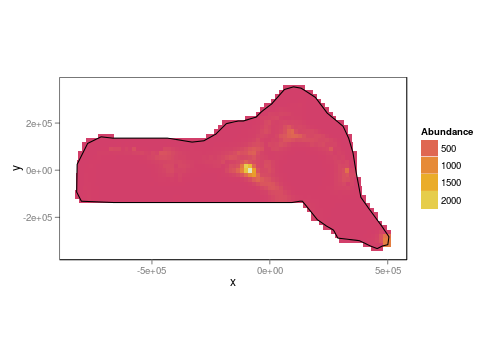
\includegraphics{mexico-figs/mod2-preds.png}
\caption{Predicted density surface for \texttt{mod2}.}
\end{figure}

Simply calling \texttt{plot} on the model object allows us to look at
the relationship between depth and abundance (shown in Figure 10):

\begin{Shaded}
\begin{Highlighting}[]
\KeywordTok{plot}\NormalTok{(mod2, }\DataTypeTok{select =} \DecValTok{2}\NormalTok{)}
\end{Highlighting}
\end{Shaded}

\begin{figure}[htbp]
\centering
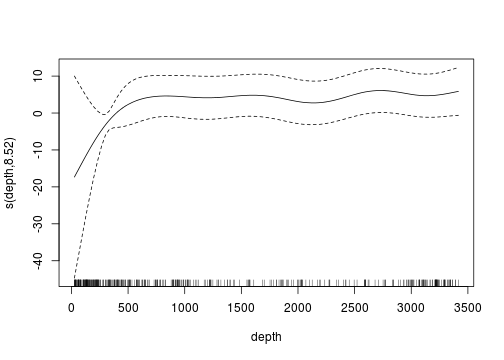
\includegraphics{mexico-figs/mod2-depth.png}
\caption{Plot of the smooth of depth in \texttt{mod2}.}
\end{figure}

Omitting the argument \texttt{select} in the call to \texttt{plot} gives
plots of all the smooth terms, one at a time.

\subsection{A more complicated model}

\textbf{\emph{Tweedie}}

Response distributions other than the quasi-Poisson can be used, for
example the Tweedie distribution. If the Tweedie is used, then the
\texttt{p} parameter must be specified. The choice of \texttt{p} is only
sensitive to the first decimal place, so a quick search can be performed
by simply comparing the score of the resulting models. In this simple
example we only show the difference between two values for \texttt{p}.

\begin{Shaded}
\begin{Highlighting}[]
\NormalTok{mod3}\FloatTok{.12} \NormalTok{<-}\StringTok{ }\KeywordTok{dsm}\NormalTok{(N ~}\StringTok{ }\KeywordTok{s}\NormalTok{(x, y), hr.model, segdata, obsdata, }
    \DataTypeTok{family =} \KeywordTok{Tweedie}\NormalTok{(}\DataTypeTok{p =}\FloatTok{1.2}\NormalTok{))}
\KeywordTok{summary}\NormalTok{(mod3}\FloatTok{.12}\NormalTok{)}
\end{Highlighting}
\end{Shaded}

\begin{verbatim}
## 
## Family: Tweedie(1.2) 
## Link function: log 
## 
## Formula:
## N ~ s(x, y) + offset(off.set)
## <environment: 0x10bb3f518>
## 
## Parametric coefficients:
##             Estimate Std. Error t value Pr(>|t|)    
## (Intercept)  -18.981      0.405   -46.9   <2e-16 ***
## ---
## Signif. codes:  0 '***' 0.001 '**' 0.01 '*' 0.05 '.' 0.1 ' ' 1
## 
## Approximate significance of smooth terms:
##         edf Ref.df    F p-value    
## s(x,y) 27.3   28.7 6.27  <2e-16 ***
## ---
## Signif. codes:  0 '***' 0.001 '**' 0.01 '*' 0.05 '.' 0.1 ' ' 1
## 
## R-sq.(adj) =  0.0531   Deviance explained = 47.9%
## GCV score = 23.284  Scale est. = 20.239    n = 387
\end{verbatim}

As well as looking at the GCV/UBRE/REML score of the model to assess the
value of \texttt{p} we can also look at a plot of the square root of the
absolute value of the residuals versus the fitted values (Figure 11,
left panel).

where as setting \texttt{p=1.7}:

\begin{Shaded}
\begin{Highlighting}[]
\NormalTok{mod3}\FloatTok{.17} \NormalTok{<-}\StringTok{ }\KeywordTok{dsm}\NormalTok{(N ~}\StringTok{ }\KeywordTok{s}\NormalTok{(x, y), hr.model, segdata, obsdata, }
    \DataTypeTok{family =} \KeywordTok{Tweedie}\NormalTok{(}\DataTypeTok{p =} \FloatTok{1.7}\NormalTok{))}
\KeywordTok{summary}\NormalTok{(mod3}\FloatTok{.17}\NormalTok{)}
\end{Highlighting}
\end{Shaded}

\begin{verbatim}
## 
## Family: Tweedie(1.7) 
## Link function: log 
## 
## Formula:
## N ~ s(x, y) + offset(off.set)
## <environment: 0x1111f2790>
## 
## Parametric coefficients:
##             Estimate Std. Error t value Pr(>|t|)    
## (Intercept)  -24.267      0.671   -36.2   <2e-16 ***
## ---
## Signif. codes:  0 '***' 0.001 '**' 0.01 '*' 0.05 '.' 0.1 ' ' 1
## 
## Approximate significance of smooth terms:
##         edf Ref.df    F p-value    
## s(x,y) 28.8     29 14.4  <2e-16 ***
## ---
## Signif. codes:  0 '***' 0.001 '**' 0.01 '*' 0.05 '.' 0.1 ' ' 1
## 
## R-sq.(adj) =  -9.81   Deviance explained = 53.4%
## GCV score = 9.3865  Scale est. = 8.0932    n = 387
\end{verbatim}

The plot (Figure 11, right panel; code below), appears to be much
flatter.

\begin{Shaded}
\begin{Highlighting}[]
\KeywordTok{par}\NormalTok{(}\DataTypeTok{mfrow =} \KeywordTok{c}\NormalTok{(}\DecValTok{1}\NormalTok{, }\DecValTok{2}\NormalTok{))}
\KeywordTok{plot}\NormalTok{(}\KeywordTok{sqrt}\NormalTok{(}\KeywordTok{abs}\NormalTok{(}\KeywordTok{residuals}\NormalTok{(mod3}\FloatTok{.12}\NormalTok{))), }\KeywordTok{predict}\NormalTok{(mod3}\FloatTok{.12}\NormalTok{), }
    \DataTypeTok{xlab =} \StringTok{"Square root of the}\CharTok{\textbackslash{}n}\StringTok{absolute value of the residuals"}\NormalTok{, }
    \DataTypeTok{ylab =} \StringTok{"Fitted values"}\NormalTok{, }\DataTypeTok{main =} \StringTok{"p=1.2"}\NormalTok{)}
\KeywordTok{plot}\NormalTok{(}\KeywordTok{sqrt}\NormalTok{(}\KeywordTok{abs}\NormalTok{(}\KeywordTok{residuals}\NormalTok{(mod3}\FloatTok{.17}\NormalTok{))), }\KeywordTok{predict}\NormalTok{(mod3}\FloatTok{.17}\NormalTok{), }
    \DataTypeTok{xlab =} \StringTok{"Square root of the}\CharTok{\textbackslash{}n}\StringTok{absolute value of the residuals"}\NormalTok{, }
    \DataTypeTok{ylab =} \StringTok{"Fitted values"}\NormalTok{, }\DataTypeTok{main =} \StringTok{"p=1.7"}\NormalTok{)}
\end{Highlighting}
\end{Shaded}

\begin{figure}[htbp]
\centering
\includegraphics{mexico-figs/tweedie-17-residplot.png}
\caption{Plot of absolute value of the residuals versus the fitted
values for the Tweedie model when \texttt{p=1.2} (left) and
\texttt{p=1.7} (right). Note that the right plot is much flatter than
the left.}
\end{figure}

Note also the improvement in GCV score.

In general, a ``good'' value can be found by simply plotting the above
along with the GCV score for the model for values of \texttt{p} between
1.1 and 1.9 and looking for the best GCV and ``flattest'' plot.

\textbf{\emph{Soap film smoothing}}

To account for a complex region (e.g., a region that includes
peninsulae) we can use the soap film smoother (Wood et al. 2008).

To use a soap film smoother for the spatial part of the model we must
create a set of knots for the smoother to use. This is easily done using
the \texttt{make.soapgrid()} function in \texttt{dsm}:

\begin{Shaded}
\begin{Highlighting}[]
\NormalTok{soap.knots <-}\StringTok{ }\KeywordTok{make.soapgrid}\NormalTok{(survey.area, }\KeywordTok{c}\NormalTok{(}\DecValTok{11}\NormalTok{, }\DecValTok{6}\NormalTok{))}
\CommentTok{# knot 11 is not outside but is too close according to soap...}
\NormalTok{soap.knots <-}\StringTok{ }\NormalTok{soap.knots[-}\DecValTok{11}\NormalTok{, ]}
\end{Highlighting}
\end{Shaded}

where the second argument specifies the number of points (in eadch
direction) in the grid that will be used to create the knots (knots in
the grid outside of \texttt{survey.area} are removed).

As we saw in the exploratory analysis, some of the transect lines are
outside of the survey area. These will cause the soap film smoother to
fail, so we remove them:

\begin{Shaded}
\begin{Highlighting}[]
\NormalTok{x <-}\StringTok{ }\NormalTok{segdata$x}
\NormalTok{y <-}\StringTok{ }\NormalTok{segdata$y}
\NormalTok{onoff <-}\StringTok{ }\KeywordTok{inSide}\NormalTok{(}\DataTypeTok{x =} \NormalTok{x, }\DataTypeTok{y =} \NormalTok{y, }\DataTypeTok{bnd =} \KeywordTok{as.list}\NormalTok{(survey.area))}
\KeywordTok{rm}\NormalTok{(x, y)}
\NormalTok{segdata.soap <-}\StringTok{ }\NormalTok{segdata[onoff, ]}
\end{Highlighting}
\end{Shaded}

We can run a model with both the \texttt{depth} covariate along with a
spatial (soap film) smooth. Note that the \texttt{k} argument now refers
to the complexity of the boundary smooth in the soap film, and the
complexity of the film is controlled by the knots given in the
\texttt{xt} argument.

\begin{Shaded}
\begin{Highlighting}[]
\NormalTok{mod4 <-}\StringTok{ }\KeywordTok{dsm}\NormalTok{(N ~}\StringTok{ }\KeywordTok{s}\NormalTok{(x, y, }\DataTypeTok{bs =} \StringTok{"so"}\NormalTok{, }\DataTypeTok{k =} \DecValTok{10}\NormalTok{, }\DataTypeTok{xt =} \KeywordTok{list}\NormalTok{(}\DataTypeTok{bnd =} \KeywordTok{list}\NormalTok{(survey.area))) +}\StringTok{ }
\StringTok{    }\KeywordTok{s}\NormalTok{(depth), hr.model, segdata.soap, obsdata, }\DataTypeTok{knots =} \NormalTok{soap.knots)}
\end{Highlighting}
\end{Shaded}

\begin{verbatim}
## Loading required package: Matrix Loading required package: lattice
\end{verbatim}

\begin{Shaded}
\begin{Highlighting}[]
\KeywordTok{summary}\NormalTok{(mod4)}
\end{Highlighting}
\end{Shaded}

\begin{verbatim}
## 
## Family: quasipoisson 
## Link function: log 
## 
## Formula:
## N ~ s(x, y, bs = "so", k = 10, xt = list(bnd = list(survey.area))) + 
##     s(depth) + offset(off.set)
## <environment: 0x10a3dfdf8>
## 
## Parametric coefficients:
##             Estimate Std. Error t value Pr(>|t|)    
## (Intercept)   -19.40       0.62   -31.3   <2e-16 ***
## ---
## Signif. codes:  0 '***' 0.001 '**' 0.01 '*' 0.05 '.' 0.1 ' ' 1
## 
## Approximate significance of smooth terms:
##            edf Ref.df    F p-value    
## s(x,y)   23.05  29.00 2.63   2e-07 ***
## s(depth)  7.08   7.89 2.57    0.01 *  
## ---
## Signif. codes:  0 '***' 0.001 '**' 0.01 '*' 0.05 '.' 0.1 ' ' 1
## 
## R-sq.(adj) =  0.183   Deviance explained = 45.9%
## GCV score = 45.227  Scale est. = 38.341    n = 365
\end{verbatim}

Comparing predictions from the model that included a smooth of depth, we
can see that the soap film has prevented some of the extreme values
(especially in the lower right corner of the survey area). This is shown
in Figure 12 (figure created with the code below).

\begin{Shaded}
\begin{Highlighting}[]
\NormalTok{mod4.pred <-}\StringTok{ }\KeywordTok{predict}\NormalTok{(mod4, preddata, off.set)}
\NormalTok{pp <-}\StringTok{ }\KeywordTok{cbind}\NormalTok{(preddata, mod4.pred)}

\NormalTok{p <-}\StringTok{ }\KeywordTok{ggplot}\NormalTok{(pp) +}\StringTok{ }\NormalTok{gg.opts}
\NormalTok{p <-}\StringTok{ }\NormalTok{p +}\StringTok{ }\KeywordTok{geom_tile}\NormalTok{(}\KeywordTok{aes}\NormalTok{(}\DataTypeTok{x =} \NormalTok{x, }\DataTypeTok{y =} \NormalTok{y, }\DataTypeTok{fill =} \NormalTok{mod4.pred, }
    \DataTypeTok{width =} \NormalTok{width, }\DataTypeTok{height =} \NormalTok{height))}
\NormalTok{p <-}\StringTok{ }\NormalTok{p +}\StringTok{ }\KeywordTok{coord_equal}\NormalTok{()}
\NormalTok{p <-}\StringTok{ }\NormalTok{p +}\StringTok{ }\KeywordTok{geom_path}\NormalTok{(}\KeywordTok{aes}\NormalTok{(}\DataTypeTok{x =} \NormalTok{x, }\DataTypeTok{y =} \NormalTok{y), }\DataTypeTok{data =} \NormalTok{survey.area)}
\NormalTok{p <-}\StringTok{ }\NormalTok{p +}\StringTok{ }\KeywordTok{labs}\NormalTok{(}\DataTypeTok{fill =} \StringTok{"Abundance"}\NormalTok{)}
\KeywordTok{print}\NormalTok{(p)}
\end{Highlighting}
\end{Shaded}

\begin{figure}[htbp]
\centering
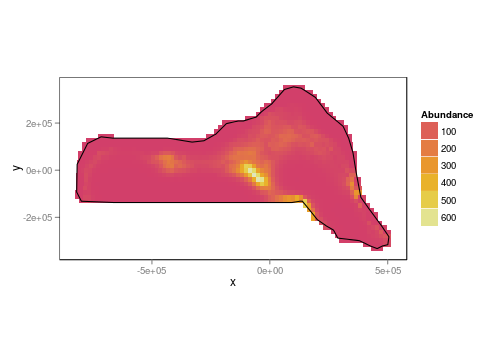
\includegraphics{mexico-figs/mod4-pred.png}
\caption{Predicted density surface for \texttt{mod4}.}
\end{figure}

\section{Adding covariates to the detection function}

It is common to include covariates in the detection function (so-called
Multiple Covariate Distance Sampling or MCDS). In this dataset there are
two covariates that were collected on each individual: Beaufort sea
state and size. For brevity we fit only a hazard-rate detection
functions with the sea state included as a factor covariate as follows:

\begin{Shaded}
\begin{Highlighting}[]
\NormalTok{hr.beau.model <-}\StringTok{ }\KeywordTok{ds}\NormalTok{(distdata, }\KeywordTok{max}\NormalTok{(distdata$distance), }
    \DataTypeTok{formula =} \NormalTok{~}\KeywordTok{as.factor}\NormalTok{(beaufort), }\DataTypeTok{key =} \StringTok{"hr"}\NormalTok{, }\DataTypeTok{adjustment =} \OtherTok{NULL}\NormalTok{)}
\KeywordTok{summary}\NormalTok{(hr.beau.model)}
\end{Highlighting}
\end{Shaded}

\begin{verbatim}
## 
## Summary for distance analysis 
## Number of observations :  47 
## Distance range         :  0  -  7847 
## 
## Model : Hazard-rate key function 
## AIC   : 843.7 
## 
## Detection function parameters
## Scale Coefficients:  
##                      estimate     se
## (Intercept)           7.66318  1.077
## as.factor(beaufort)2  2.27968 17.367
## as.factor(beaufort)3  0.28606  1.019
## as.factor(beaufort)4  0.07174  1.223
## as.factor(beaufort)5 -0.36399  1.537
## 
## Shape parameters:  
##             estimate    se
## (Intercept)   0.3004 0.518
## 
##                     Estimate      SE     CV
## Average p             0.5421  0.1751 0.3229
## N in covered region  86.6957 29.4133 0.3393
\end{verbatim}

In this example, the detection function with covariates does not give a
lower AIC than the model without covariates (hazard-rate model has AIC
of 841.25 vs.~843.71 for this model). Looking back to the bottom-right
panel of Figure 2, we can see there is not a discernible pattern in the
plot of Beaufort vs distance.

The code to fit the model is similar to the other models, above. However
since we are now using a detection function with observation-level
covariates, we change the response to be \texttt{Nhat} so the abundances
are estimated per segment and change the name ofthe detection function
model object:

\begin{Shaded}
\begin{Highlighting}[]
\NormalTok{mod5 <-}\StringTok{ }\KeywordTok{dsm}\NormalTok{(Nhat ~}\StringTok{ }\KeywordTok{s}\NormalTok{(x, y), hr.beau.model, segdata, obsdata)}
\KeywordTok{summary}\NormalTok{(mod5)}
\end{Highlighting}
\end{Shaded}

\begin{verbatim}
## 
## Family: quasipoisson 
## Link function: log 
## 
## Formula:
## Nhat ~ s(x, y) + offset(off.set)
## <environment: 0x107da5320>
## 
## Parametric coefficients:
##             Estimate Std. Error t value Pr(>|t|)    
## (Intercept)  -18.258      0.351     -52   <2e-16 ***
## ---
## Signif. codes:  0 '***' 0.001 '**' 0.01 '*' 0.05 '.' 0.1 ' ' 1
## 
## Approximate significance of smooth terms:
##        edf Ref.df    F p-value    
## s(x,y)  26   28.1 5.77  <2e-16 ***
## ---
## Signif. codes:  0 '***' 0.001 '**' 0.01 '*' 0.05 '.' 0.1 ' ' 1
## 
## R-sq.(adj) =  0.118   Deviance explained = 42.9%
## GCV score =  75.24  Scale est. = 65.855    n = 387
\end{verbatim}

Note that for models where there are covariates at the individual level
we cannot calculate the variance via the variance propagation method
(\texttt{dsm.var.prop}) of Williams et al (2011). Instead we can use a
GAM uncertainty estimation and combine it with the detection function
uncertainty via the delta method (\texttt{dsm.var.gam}), or use the
moving block bootstrap. Other than this, all of the above functions can
be used.

A plot of predictions from the covariate model:

\begin{Shaded}
\begin{Highlighting}[]
\NormalTok{mod5.pred <-}\StringTok{ }\KeywordTok{predict}\NormalTok{(mod5, preddata, off.set)}
\NormalTok{pp <-}\StringTok{ }\KeywordTok{cbind}\NormalTok{(preddata, mod5.pred)}

\NormalTok{p <-}\StringTok{ }\KeywordTok{ggplot}\NormalTok{(pp) +}\StringTok{ }\NormalTok{gg.opts}
\NormalTok{p <-}\StringTok{ }\NormalTok{p +}\StringTok{ }\KeywordTok{geom_tile}\NormalTok{(}\KeywordTok{aes}\NormalTok{(}\DataTypeTok{x =} \NormalTok{x, }\DataTypeTok{y =} \NormalTok{y, }\DataTypeTok{fill =} \NormalTok{mod5.pred, }
    \DataTypeTok{width =} \NormalTok{width, }\DataTypeTok{height =} \NormalTok{height))}
\NormalTok{p <-}\StringTok{ }\NormalTok{p +}\StringTok{ }\KeywordTok{coord_equal}\NormalTok{()}
\NormalTok{p <-}\StringTok{ }\NormalTok{p +}\StringTok{ }\KeywordTok{geom_path}\NormalTok{(}\KeywordTok{aes}\NormalTok{(}\DataTypeTok{x =} \NormalTok{x, }\DataTypeTok{y =} \NormalTok{y), }\DataTypeTok{data =} \NormalTok{survey.area)}
\NormalTok{p <-}\StringTok{ }\NormalTok{p +}\StringTok{ }\KeywordTok{labs}\NormalTok{(}\DataTypeTok{fill =} \StringTok{"Abundance"}\NormalTok{)}
\KeywordTok{print}\NormalTok{(p)}
\end{Highlighting}
\end{Shaded}

\begin{figure}[htbp]
\centering
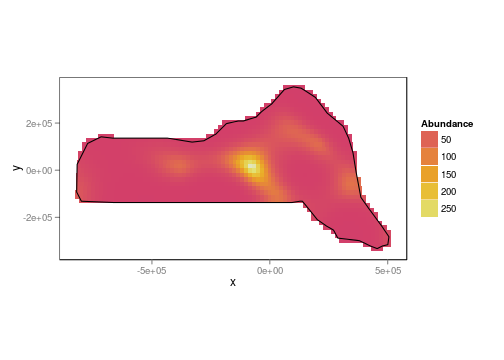
\includegraphics{mexico-figs/mod5-pred.png}
\caption{Predicted density surface for \texttt{mod5}.}
\end{figure}

\section{Correlation structures}

We can use a generalized mixed model (GAMM; Wood, 2006) to include
correlation between the segments within each transect. First we re-code
the sample labels and transect labels as numeric variables, then include
them in the model as part of the \texttt{correlation} argument. For the
sake of example we use an AR1 (lag 1 autocorrelation) correlation
structure (though the correlogram did not indicate we had issues with
residual autocorrelation, we show it here for illustrative purposes).

\begin{Shaded}
\begin{Highlighting}[]
\NormalTok{segdata$sg.id <-}\StringTok{ }\KeywordTok{as.numeric}\NormalTok{(segdata$Sample.Label)}
\NormalTok{segdata$tr.id <-}\StringTok{ }\KeywordTok{as.numeric}\NormalTok{(segdata$Transect.Label)}
\NormalTok{mod1.gamm <-}\StringTok{ }\KeywordTok{dsm}\NormalTok{(N ~}\StringTok{ }\KeywordTok{s}\NormalTok{(x, y), hr.model$ddf, segdata, obsdata, }\DataTypeTok{engine =} \StringTok{"gamm"}\NormalTok{, }
    \DataTypeTok{correlation =} \KeywordTok{corAR1}\NormalTok{(}\DataTypeTok{form =} \NormalTok{~sg.id), }\DataTypeTok{method =} \StringTok{"REML"}\NormalTok{)}
\end{Highlighting}
\end{Shaded}

\begin{verbatim}
## Loading required package: nlme
\end{verbatim}

\begin{verbatim}
## 
##  Maximum number of PQL iterations:  20
\end{verbatim}

\begin{verbatim}
## iteration 1 iteration 2 iteration 3 iteration 4 iteration 5 iteration 6
## iteration 7 iteration 8 iteration 9 iteration 10
\end{verbatim}

This example also includes using \texttt{method="REML"} for smoothing
parameter selection.

GAMMs usually take considerably longer to fit than GAMs, so it's usually
start with a GAM first, select smooth terms and response distribution
before starting to fit GAMMs.

The object returned is part \texttt{lme} (for the random effects) and
part \texttt{gam} (for the smooth terms). Looking at the
\texttt{summary()} for the \texttt{gam} part of the model:

\begin{Shaded}
\begin{Highlighting}[]
\KeywordTok{summary}\NormalTok{(mod1.gamm$gam)}
\end{Highlighting}
\end{Shaded}

\begin{verbatim}
## 
## Family: quasipoisson 
## Link function: log 
## 
## Formula:
## N ~ s(x, y) + offset(off.set)
## <environment: 0x108fb1ed0>
## 
## Parametric coefficients:
##             Estimate Std. Error t value Pr(>|t|)    
## (Intercept)  -17.617      0.277   -63.5   <2e-16 ***
## ---
## Signif. codes:  0 '***' 0.001 '**' 0.01 '*' 0.05 '.' 0.1 ' ' 1
## 
## Approximate significance of smooth terms:
##         edf Ref.df    F p-value    
## s(x,y) 20.4   20.4 4.08 1.5e-08 ***
## ---
## Signif. codes:  0 '***' 0.001 '**' 0.01 '*' 0.05 '.' 0.1 ' ' 1
## 
## R-sq.(adj) =  0.129  Scale est. = 68.686    n = 387
\end{verbatim}

And run checks on the GAM part of the object (shown in Figure 14):

\begin{Shaded}
\begin{Highlighting}[]
\KeywordTok{gam.check}\NormalTok{(mod1.gamm$gam)}
\end{Highlighting}
\end{Shaded}

\begin{figure}[htbp]
\centering
\includegraphics{mexico-figs/mod1-gamm-check.png}
\caption{Diagnostic plots for \texttt{mod1.gamm}.}
\end{figure}

We can now make predictions and compare the abundance map produced by
this model to the previous models (Figure 15):

\begin{Shaded}
\begin{Highlighting}[]
\NormalTok{mod1.gamm.pred <-}\StringTok{ }\KeywordTok{predict}\NormalTok{(mod1.gamm, preddata, off.set)}
\NormalTok{pp <-}\StringTok{ }\KeywordTok{cbind}\NormalTok{(preddata, }\DataTypeTok{N =} \NormalTok{mod1.gamm.pred)}
\NormalTok{p <-}\StringTok{ }\KeywordTok{ggplot}\NormalTok{(pp) +}\StringTok{ }\NormalTok{gg.opts}
\NormalTok{p <-}\StringTok{ }\NormalTok{p +}\StringTok{ }\KeywordTok{geom_tile}\NormalTok{(}\KeywordTok{aes}\NormalTok{(}\DataTypeTok{x =} \NormalTok{x, }\DataTypeTok{y =} \NormalTok{y, }\DataTypeTok{fill =} \NormalTok{N, }\DataTypeTok{width =} \NormalTok{width, }\DataTypeTok{height =} \NormalTok{height))}
\NormalTok{p <-}\StringTok{ }\NormalTok{p +}\StringTok{ }\KeywordTok{coord_equal}\NormalTok{()}
\NormalTok{p <-}\StringTok{ }\NormalTok{p +}\StringTok{ }\KeywordTok{geom_path}\NormalTok{(}\KeywordTok{aes}\NormalTok{(}\DataTypeTok{x =} \NormalTok{x, }\DataTypeTok{y =} \NormalTok{y), }\DataTypeTok{data =} \NormalTok{survey.area)}
\NormalTok{p <-}\StringTok{ }\NormalTok{p +}\StringTok{ }\KeywordTok{labs}\NormalTok{(}\DataTypeTok{fill =} \StringTok{"Abundance"}\NormalTok{)}
\KeywordTok{print}\NormalTok{(p)}
\end{Highlighting}
\end{Shaded}

\begin{figure}[htbp]
\centering
\includegraphics{mexico-figs/mod1-gamm-preds.png}
\caption{Predicted density surface for \texttt{mod1.gamm}.}
\end{figure}

Again, estimating variance is straightforward using the variance
propagation method:

\begin{Shaded}
\begin{Highlighting}[]
\NormalTok{mod1.gamm.var <-}\StringTok{ }\KeywordTok{dsm.var.prop}\NormalTok{(mod1.gamm, }\DataTypeTok{pred.data =} \NormalTok{preddata, }\DataTypeTok{off.set =} \NormalTok{off.set)}
\end{Highlighting}
\end{Shaded}

\begin{verbatim}
## 
##  Maximum number of PQL iterations:  20
\end{verbatim}

\begin{verbatim}
## iteration 1 iteration 2 iteration 3 iteration 4 iteration 5 iteration 6
## iteration 7 iteration 8 iteration 9
\end{verbatim}

\begin{Shaded}
\begin{Highlighting}[]
\KeywordTok{summary}\NormalTok{(mod1.gamm.var)}
\end{Highlighting}
\end{Shaded}

\begin{verbatim}
## Summary of uncertainty in a density surface model calculated
##  by variance propagation.
## 
## Quantiles of differences between fitted model and variance model
##    Min. 1st Qu.  Median    Mean 3rd Qu.    Max. 
##  -4.120  -0.531  -0.244  -0.073  -0.019  19.500 
## 
## Approximate asymptotic confidence interval:
##    5%  Mean   95% 
## 35389 45701 59018 
## (Using delta method)
## 
## Point estimate                 : 45701 
## Standard error                 : 5988 
## Coefficient of variation       : 0.131
\end{verbatim}

Comparing this to the variance from \texttt{mod1}, we can see the GAMM
offers a significant reduction in variance:

\begin{Shaded}
\begin{Highlighting}[]
\NormalTok{mod1.varprop <-}\StringTok{ }\KeywordTok{dsm.var.prop}\NormalTok{(mod1, }\DataTypeTok{pred.data =} \NormalTok{preddata.varprop, }
    \DataTypeTok{off.set =} \NormalTok{offset.varprop)}
\KeywordTok{summary}\NormalTok{(mod1.varprop)}
\end{Highlighting}
\end{Shaded}

\begin{verbatim}
## Summary of uncertainty in a density surface model calculated
##  by variance propagation.
## 
## Quantiles of differences between fitted model and variance model
##      Min.   1st Qu.    Median      Mean   3rd Qu.      Max. 
## -6.57e-13 -1.00e-15  1.20e-14  1.08e-13  1.11e-13  3.67e-12 
## 
## Approximate asymptotic confidence interval:
##    5%  Mean   95% 
## 29962 47034 73832 
## (Using delta method)
## 
## Point estimate                 : 47034 
## Standard error                 : 10966 
## Coefficient of variation       : 0.2331
\end{verbatim}

More information on \texttt{lme} can be found in Pinheiro and Bates
(2000) and Wood (2006).

\section{Conclusions}

This document has shown that the \texttt{dsm} package is a versatile and
relatively easy-to-use package for the analysis of spatial distance
sampling data. Note that there are many possible models that can be
fitted using \texttt{dsm} and that the aim here was to show just a few
of the options. Results from the models can be rather different, so care
must be taken in performing model selection, discrimination and
criticism.

\section*{Notes}

\begin{itemize}
\itemsep1pt\parskip0pt\parsep0pt
\item
  \texttt{Distance} is available at
  \url{http://github.com/dill/Distance} as well as on CRAN.
\item
  \texttt{dsm} is available (along with some documentation and hints) at
  \url{http://github.com/dill/dsm}, as well as on CRAN.
\end{itemize}

\section*{References}

\begin{itemize}
\itemsep1pt\parskip0pt\parsep0pt
\item
  Hedley, S.L. \& Buckland, S.T. (2004) Spatial models for line transect
  sampling. Journal of Agricultural, Biological, and Environmental
  Statistics, 9, 181--199.
\item
  Pinheiro, J.C., and Bates, D.M. (2000) Mixed-effects models in S and
  S-PLUS, Springer.
\item
  Williams, R., Hedley, S.L., Branch, T.A., Bravington, M.V., Zerbini,
  A.N. \& Findlay, K.P. (2011) Chilean blue whales as a case study to
  illustrate methods to estimate abundance and evaluate conservation
  status of rare species. Conservation Biology, 25, 526--535.
\item
  Wood, S.N. (2006) Generalized Additive Models: an introduction with R.
  Chapman and Hall/CRC Press.
\end{itemize}

\end{document}
